\subsection{Coxeter 矩阵与 Coxeter 图}

定义 4. 设 I 为一个集合。I 型 Coxeter 矩阵是一个对称方阵 \(\mathrm{M} = (m_{ij})_{i,j\in \mathrm{I}}\)，其元素为整数或 \(+\infty\)，并满足关系

\[
m _ {i i} = 1 \quad \text {   for   all   } i \in \mathrm{I};\tag{25}
\]

\[
m _ {i j} \geqslant 2 \quad \text {   for   } i, j \in I \text {   with   } i \neq j.\tag{26}
\]

I 型 Coxeter 图是（滥用术语而言）如下的一个对：一个图 \(\Gamma^{3}\)，其顶点集为 I；以及从该图的边集到由 \(+\infty\) 和所有 \(\geqslant 3\) 的整数构成的集合的一个映射 f。\(\Gamma\) 称为 Coxeter 图 \((\Gamma, f)\) 的底图。

每个 I 型 Coxeter 矩阵的 Coxeter 图 \((\Gamma, f)\) 都与矩阵 \(M\) 相关联，如下所述：

图 \(\Gamma\) 的顶点集为 I，边集为由 I 中元素组成的二元集合 \(\{i,j\}\) 的集合，其中满足 \(m_{ij} \geqslant 3\)，而映射 \(f\) 将边 \(\{i,j\}\) 关联到 M 中相应的元素 \(m_{ij}\)。

显然，这在 I 型 Coxeter 矩阵集合与 I 型 Coxeter 图集合之间给出了一个双射。

为了帮助读者理解我们的论证，我们常常用表示其底图的图示来表示 I 型 Coxeter 图，并在每条边 \(\{i,j\}\) 旁边或上方写出数值 \(f(\{i,j\})\)。如果这些数等于 3，我们通常省略它们。

若 (W,S) 是一个 Coxeter 系统，则矩阵 \(M = (m(s,s'))_{s,s' \in S}\)，其中 \(m(s,s')\) 是 \(ss'\) 的阶，是 S 型 Coxeter 矩阵，称为 (W,S) 的 Coxeter 矩阵：事实上，\(m(s,s) = 1\)，因为 \(s^2 = 1\) 对所有 \(s \in S\) 成立；且 \(m(s,s') = m(s',s) \geqslant 2\) 当 \(s \neq s'\) 时，因为 \(ss' = (s's)^{-1}\) 且 \(\neq 1\)。与 M 相关联的 Coxeter 图 \((\Gamma, f)\) 称为 (W,S) 的 Coxeter 图。我们注意到，两个顶点 \(s\) 和 \(s'\) 属于 \(\Gamma\) 当且仅当 \(s\) 和 \(s'\) 不交换。例如，阶为 \(2m\) 的二面体群的 Coxeter 矩阵为 \(\begin{pmatrix} 1 & m \\ m & 1 \end{pmatrix}\)，其 Coxeter 图表示为

当 \(m \geqslant 3\) 时（或者

\pandocbounded{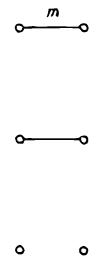
\includegraphics[keepaspectratio]{images/part001_5ff7a109.jpg}}

当 \(m = 3\) 时），而在

当 \(m = 2\) 时。*对称群 \(\mathfrak{S}_n\) 的 Coxeter 图表示为

\pandocbounded{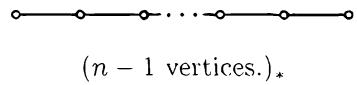
\includegraphics[keepaspectratio]{images/part001_1071b0ee.jpg}}

我们将在后面（第 V 章，第 4 节）证明，反过来，每个 Coxeter 矩阵都是某个 Coxeter 系统的矩阵。

如果 Coxeter 图的底图连通（附录，第 2 号）且非空，则称 Coxeter 系统 \((W,S)\) 是不可约的。等价地，S 非空，并且不存在将 S 划分为两个不同子集 \(S'\) 和 \(S''\) 的划分，使得 \(S'\) 的每个元素都与 \(S''\) 的每个元素交换。更一般地，设 \((\Gamma_{i})_{i\in I}\) 为 \(\Gamma\) 的连通分支族（附录，第 2 号），并设 \(S_{i}\) 为 \(\Gamma_{i}\) 的顶点集。令 \(W_{i}=W_{S_i}\) 为由 \(S_{i}\) 生成的 W 的子群（参见第 8 号）。于是 \((W_{i},S_{i})\) 是不可约 Coxeter 系统（第 8 号，定理 2），称为 \((W,S)\) 的不可约分支。此外，群 W 是限制直积 \(^{4}\)，其因子为子群 \(W_{i}\)（其中 \(i\in I\)）。事实上，这由下面更一般的命题得到：

命题 8. 设 \((\mathrm{S}_{i})_{i\in\mathrm{I}}\) 是 S 的一个划分，使得 \(S_{i}\) 的每个元素都与 \(S_{j}\) 的每个元素交换，只要 \(i\neq j\)。对于所有 \(i\in I\)，令 \(W_{i}\) 为由 \(S_{i}\) 生成的子群。于是 W 是族 \((\mathrm{W}_{i})_{i\in\mathrm{I}}\) 的限制直积。

显然，对于所有 \(i \in I\)，子群 \(W_i'\) 由 \(W_j\)（其中 \(j \neq i\)）的并生成，也由 \(S_i' = \bigcup_{i \neq j} S_j\) 生成。因此

\[
\mathrm{W} _ {i} \cap \mathrm{W} _ {i} ^ {\prime} = \mathrm{W} _ {\varnothing} = \{1 \}
\]

由第 8 号的定理 2。由于 W 由各 \(W_{i}\) 的并生成，命题得证。

